\documentclass[11pt]{article}

\usepackage[margin=1in]{geometry}
\usepackage{listings}
\usepackage{xcolor}
\usepackage{hyperref}
\usepackage{enumitem}
\usepackage{booktabs}
\usepackage{graphicx}
\usepackage{tikz}
\usetikzlibrary{arrows.meta, positioning, shapes.geometric}

\hypersetup{
    colorlinks=true,
    linkcolor=blue,
    urlcolor=blue
}

\lstset{
    backgroundcolor=\color{gray!10},
    basicstyle=\ttfamily\small,
    breaklines=true,
    frame=single,
    rulecolor=\color{gray!40},
    xleftmargin=6pt,
    xrightmargin=6pt,
    aboveskip=10pt,
    belowskip=10pt,
    columns=fullflexible,
    keepspaces=true
}

\lstdefinestyle{yaml}{
    basicstyle=\ttfamily\small,
    commentstyle=\color{gray},
    morecomment=[l]{\#},
}

\lstdefinestyle{error}{
    basicstyle=\ttfamily\small\color{red!70!black},
    backgroundcolor=\color{red!5},
    rulecolor=\color{red!40},
}

\title{Nav2 Bringup Troubleshooting\\[4pt]
\large AVROS Ackermann Vehicle~|~ROS2 Humble~|~GPS Navigation}
\author{AVROS Team}
\date{March 2026}

\begin{document}
\maketitle
\tableofcontents
\newpage

\section{Introduction}

This document records the problems encountered while bringing up the Nav2 navigation stack on the AVROS platform---an Ackermann-steered autonomous vehicle running ROS2 Humble on an NVIDIA Jetson Orin. The vehicle uses:

\begin{itemize}[nosep]
    \item \textbf{LiDAR:} Velodyne VLP-16
    \item \textbf{Camera:} Intel RealSense D455
    \item \textbf{IMU + GNSS:} Xsens MTi-680G
    \item \textbf{Localization:} robot\_localization (dual EKF) + navsat\_transform
    \item \textbf{Navigation:} Nav2 (SmacPlannerHybrid, Regulated Pure Pursuit)
    \item \textbf{Actuation:} Teensy MCU via UDP (Ackermann steering)
\end{itemize}

Each section describes one problem, the error message, root cause analysis, and the fix applied. Problems are presented in the order they were encountered during bringup.

%% ============================================================
\section{Nav2 Plugin Name Format Mismatch}
\label{sec:plugin-names}

\subsection{Symptom}

Nav2 nodes crash at startup with \texttt{FATAL} errors indicating that a plugin ``does not exist,'' even though the plugin package is installed.

\begin{lstlisting}[style=error]
[controller_server] [FATAL]: Failed to create progress_checker.
  Exception: According to the loaded plugin descriptions the class
  nav2_controller/SimpleProgressChecker does not exist.
  Declared types are nav2_controller::SimpleProgressChecker
\end{lstlisting}

\subsection{Root Cause}

Nav2 plugins in ROS2 Humble use \textbf{two different separator formats} in \texttt{plugin:} fields depending on how the plugin is declared in its XML registration file:

\begin{itemize}
    \item Plugins declared with an explicit \texttt{class name="..."} attribute in their \texttt{plugin.xml} use the \textbf{slash} format: \texttt{namespace/ClassName}
    \item Plugins declared with only \texttt{class type="..."} use the \textbf{double-colon} format: \texttt{namespace::ClassName}
\end{itemize}

This is not documented in the Nav2 configuration guides and must be determined by inspecting the actual plugin XML files installed on the system.

\subsection{Investigation}

The correct format for each plugin was determined by examining the XML files on the Jetson:

\begin{lstlisting}
# Example: SmacPlannerHybrid uses slash (has class name=)
grep -r "SmacPlannerHybrid" /opt/ros/humble/share/nav2_smac_planner/

# Example: SimpleProgressChecker uses :: (no class name=)
grep -r "SimpleProgressChecker" /opt/ros/humble/share/nav2_controller/
\end{lstlisting}

\subsection{Correct Plugin Formats}

\begin{table}[h]
\centering
\begin{tabular}{@{}lll@{}}
    \toprule
    Plugin & Correct Format & Separator \\
    \midrule
    SimpleProgressChecker & \texttt{nav2\_controller::SimpleProgressChecker} & \texttt{::} \\
    SimpleGoalChecker & \texttt{nav2\_controller::SimpleGoalChecker} & \texttt{::} \\
    RegulatedPurePursuitController & \texttt{nav2\_regulated\_pure\_pursuit\_controller::...} & \texttt{::} \\
    SmacPlannerHybrid & \texttt{nav2\_smac\_planner/SmacPlannerHybrid} & \texttt{/} \\
    SimpleSmoother & \texttt{nav2\_smoother::SimpleSmoother} & \texttt{::} \\
    BackUp & \texttt{nav2\_behaviors/BackUp} & \texttt{/} \\
    DriveOnHeading & \texttt{nav2\_behaviors/DriveOnHeading} & \texttt{/} \\
    Wait & \texttt{nav2\_behaviors/Wait} & \texttt{/} \\
    NavigateToPoseNavigator & \texttt{nav2\_bt\_navigator::NavigateToPoseNavigator} & \texttt{::} \\
    NavigateThroughPosesNavigator & \texttt{nav2\_bt\_navigator::NavigateThroughPosesNavigator} & \texttt{::} \\
    \bottomrule
\end{tabular}
\caption{Nav2 plugin name formats (ROS2 Humble)}
\label{tab:plugin-formats}
\end{table}

\subsection{Lesson}

Do not assume a uniform separator format across Nav2 plugins. When encountering ``class does not exist'' errors, inspect the plugin XML files under \texttt{/opt/ros/humble/share/<package>/} on the target system. The error message itself lists the declared types in the correct format.

%% ============================================================
\section{Invalid SmacPlannerHybrid Parameters}
\label{sec:smac-params}

\subsection{Symptom}

Two issues with SmacPlannerHybrid configuration parameters:

\begin{enumerate}
    \item \texttt{cost\_travel\_multiplier} --- parameter accepted silently but has no effect
    \item \texttt{reversing\_penalty} --- parameter name incorrect, causes unexpected planner behavior
\end{enumerate}

\subsection{Root Cause}

\begin{itemize}
    \item \texttt{cost\_travel\_multiplier} is a parameter for \texttt{SmacPlanner2D}, not \texttt{SmacPlannerHybrid}. ROS2 parameters are not type-checked across plugins---unknown parameters are silently ignored.
    \item The correct parameter name is \texttt{reverse\_penalty}, not \texttt{reversing\_penalty}. This was a naming discrepancy between documentation versions.
\end{itemize}

\subsection{Fix}

\begin{lstlisting}[style=yaml]
# WRONG
GridBased:
  plugin: "nav2_smac_planner/SmacPlannerHybrid"
  cost_travel_multiplier: 2.0    # belongs to SmacPlanner2D
  reversing_penalty: 2.0         # wrong parameter name

# CORRECT
GridBased:
  plugin: "nav2_smac_planner/SmacPlannerHybrid"
  reverse_penalty: 2.0           # correct name for Hybrid
\end{lstlisting}

\subsection{Lesson}

Always verify parameter names against the source code or the official Nav2 API documentation for the specific planner variant in use. ROS2 does not warn about unused parameters by default.

%% ============================================================
\section{Missing \texttt{map} Frame --- Single EKF Architecture}
\label{sec:missing-map}

\subsection{Symptom}

After launching the navigation stack, Nav2 nodes wait indefinitely for the \texttt{map} frame:

\begin{lstlisting}[style=error]
[planner_server] Timed out waiting for transform.
  Could not transform from "base_link" to "map".
  "map" frame does not exist.
\end{lstlisting}

The TF tree only contained \texttt{odom $\to$ base\_link}. The navsat\_transform\_node was publishing a \texttt{utm} frame instead of \texttt{map}.

\subsection{Root Cause}

The initial localization setup used a \textbf{single EKF} with \texttt{world\_frame: odom}. This EKF published only the \texttt{odom $\to$ base\_link} transform. The navsat\_transform\_node converts GPS to Cartesian odometry but its \texttt{broadcast\_cartesian\_transform} publishes a \texttt{utm} frame---it does not publish a \texttt{map} frame.

No node was responsible for publishing the \texttt{map $\to$ odom} transform that Nav2 requires.

\subsection{Fix: Dual EKF Architecture}

The standard approach for GPS-based navigation with Nav2, documented in the \href{https://github.com/ros-navigation/navigation2_tutorials/tree/master/nav2_gps_waypoint_follower_demo}{nav2\_gps\_waypoint\_follower\_demo}, uses \textbf{two EKF instances}:

\begin{figure}[h]
\centering
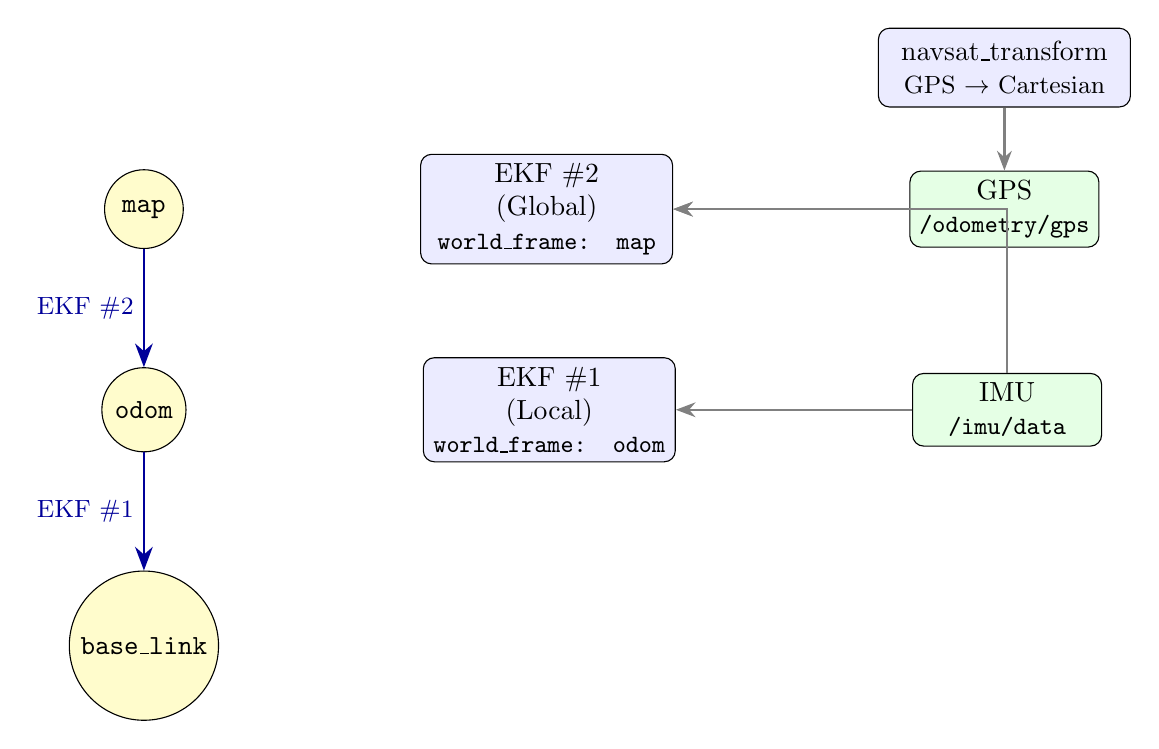
\begin{tikzpicture}[
    node distance=1.8cm,
    block/.style={draw, rounded corners, minimum width=3.2cm, minimum height=1cm, align=center, fill=blue!8},
    sensor/.style={draw, rounded corners, minimum width=2.4cm, minimum height=0.8cm, align=center, fill=green!10},
    tf/.style={-{Stealth[length=3mm]}, thick, blue!60!black},
    data/.style={-{Stealth[length=2.5mm]}, thick, gray},
]

% TF frames
\node[draw, circle, fill=yellow!20, minimum size=1cm] (map) {\texttt{map}};
\node[draw, circle, fill=yellow!20, minimum size=1cm, below=1.5cm of map] (odom) {\texttt{odom}};
\node[draw, circle, fill=yellow!20, minimum size=1cm, below=1.5cm of odom] (base) {\texttt{base\_link}};

% EKF nodes
\node[block, right=3cm of map] (ekf2) {EKF \#2\\(Global)\\{\small\texttt{world\_frame: map}}};
\node[block, right=3cm of odom] (ekf1) {EKF \#1\\(Local)\\{\small\texttt{world\_frame: odom}}};

% Sensors
\node[sensor, right=3cm of ekf2] (gps) {GPS\\{\small\texttt{/odometry/gps}}};
\node[sensor, right=3cm of ekf1] (imu) {IMU\\{\small\texttt{/imu/data}}};

% navsat
\node[block, above=0.8cm of gps] (navsat) {navsat\_transform\\{\small GPS $\to$ Cartesian}};

% TF arrows
\draw[tf] (map) -- node[left, font=\small] {EKF \#2} (odom);
\draw[tf] (odom) -- node[left, font=\small] {EKF \#1} (base);

% Data arrows
\draw[data] (imu) -- (ekf1);
\draw[data] (imu) |- (ekf2);
\draw[data] (gps) -- (ekf2);
\draw[data] (navsat) -- (gps);

\end{tikzpicture}
\caption{Dual EKF architecture for GPS-based navigation}
\label{fig:dual-ekf}
\end{figure}

\begin{itemize}
    \item \textbf{EKF \#1} (local): \texttt{world\_frame: odom}. Fuses IMU only. Publishes \texttt{odom $\to$ base\_link}. Output topic: \texttt{/odometry/filtered} (used by Nav2 controller and local costmap).
    \item \textbf{EKF \#2} (global): \texttt{world\_frame: map}. Fuses IMU + GPS odometry from navsat\_transform. Publishes \texttt{map $\to$ odom}. Output topic: \texttt{/odometry/global} (consumed by navsat\_transform).
    \item \textbf{navsat\_transform}: Converts GPS (\texttt{NavSatFix}) to Cartesian odometry (\texttt{/odometry/gps}) for EKF \#2. Reads the global EKF output (\texttt{/odometry/global}) for its internal reference.
\end{itemize}

\subsubsection{EKF Configuration (\texttt{ekf.yaml})}

\begin{lstlisting}[style=yaml]
# --- Local EKF: odom -> base_link ---
ekf_filter_node_odom:
  ros__parameters:
    frequency: 30.0
    two_d_mode: true
    publish_tf: true
    map_frame: map
    odom_frame: odom
    base_link_frame: base_link
    world_frame: odom           # key difference

    imu0: /imu/data
    imu0_config: [false, false, false,
                  true,  true,  true,
                  false, false, false,
                  true,  true,  true,
                  false, false, false]
    imu0_remove_gravitational_acceleration: true

# --- Global EKF: map -> odom ---
ekf_filter_node_map:
  ros__parameters:
    frequency: 30.0
    two_d_mode: true
    publish_tf: true
    map_frame: map
    odom_frame: odom
    base_link_frame: base_link
    world_frame: map            # key difference

    imu0: /imu/data
    imu0_config: [false, false, false,
                  true,  true,  true,
                  false, false, false,
                  true,  true,  true,
                  false, false, false]
    imu0_remove_gravitational_acceleration: true

    odom0: /odometry/gps        # GPS input from navsat_transform
    odom0_config: [true,  true,  false,
                   false, false, false,
                   false, false, false,
                   false, false, false,
                   false, false, false]
\end{lstlisting}

\subsubsection{Launch File Remappings}

The two EKF nodes share the same config file but are distinguished by node name (which selects the correct YAML section) and output topic remappings:

\begin{lstlisting}[style=yaml]
# EKF #1 output -> /odometry/filtered (for Nav2)
Node(name='ekf_filter_node_odom',
     remappings=[('odometry/filtered', '/odometry/filtered')])

# EKF #2 output -> /odometry/global (for navsat_transform)
Node(name='ekf_filter_node_map',
     remappings=[('odometry/filtered', '/odometry/global')])

# navsat_transform reads /odometry/global, publishes /odometry/gps
Node(name='navsat_transform',
     remappings=[
         ('odometry/filtered', '/odometry/global'),
         ('odometry/gps', '/odometry/gps'),
         ('gps/fix', '/gnss'),
     ])
\end{lstlisting}

\subsection{Lesson}

For GPS-based navigation with Nav2, a single EKF is insufficient. The standard dual EKF pattern from the \texttt{nav2\_gps\_waypoint\_follower\_demo} tutorial must be used. The local EKF provides smooth, drift-free odometry for the controller, while the global EKF anchors the robot's position in the \texttt{map} frame using GPS.

%% ============================================================
\section{Xsens \texttt{pub\_gnsspose} TF Loop}
\label{sec:xsens-tf}

\subsection{Symptom}

After launching the Xsens driver alongside the dual EKF, a TF loop appeared:

\begin{lstlisting}[style=error]
[robot_state_publisher] TF_REPEATED_DATA ignoring data with
  redundant timestamp. Link: imu_link -> base_link
\end{lstlisting}

The Xsens driver was publishing a \texttt{imu\_link $\to$ base\_link} transform that conflicted with the URDF-defined static transform (published by robot\_state\_publisher).

\subsection{Root Cause}

The Xsens MTi-680G ROS2 driver parameter \texttt{pub\_gnsspose: true} causes the driver to publish its own TF transform from sensor frame to base frame, creating a conflict with the URDF's static transform and introducing a TF loop into the tree.

\subsection{Fix}

Disable \texttt{pub\_gnsspose} in \texttt{xsens.yaml}:

\begin{lstlisting}[style=yaml]
xsens_mti_node:
  ros__parameters:
    pub_gnsspose: false   # Disable -- creates TF loop with EKF + URDF
\end{lstlisting}

The URDF (\texttt{avros.urdf.xacro}) defines the static \texttt{base\_link $\to$ imu\_link} transform, which is published by \texttt{robot\_state\_publisher}. The Xsens driver should only publish sensor data, not TF transforms.

%% ============================================================
\section{BT Navigator Spin Recovery Failure (Ackermann Vehicle)}
\label{sec:bt-spin}

\subsection{Symptom}

The \texttt{bt\_navigator} node fails to activate:

\begin{lstlisting}[style=error]
[bt_navigator] Action server "spin" not available after waiting.
  Navigation cannot proceed. Shutting down.
\end{lstlisting}

\subsection{Root Cause}

The default Nav2 behavior tree XML (\texttt{navigate\_to\_pose\_w\_replanning\_and\_recovery.xml}) includes a \texttt{<Spin>} recovery action. This action requires a \texttt{spin} behavior plugin in the behavior\_server. However, an Ackermann-steered vehicle \textbf{cannot rotate in place}---the spin recovery is physically impossible.

Adding a spin plugin to the behavior\_server would be incorrect, as the behavior would never succeed and would block recovery indefinitely.

\subsection{Fix}

Use a behavior tree XML that does not include spin or in-place rotation recovery. Nav2 ships with \texttt{navigate\_w\_replanning\_only\_if\_path\_becomes\_invalid.xml}, which replans without attempting spin recovery:

\begin{lstlisting}[style=yaml]
bt_navigator:
  ros__parameters:
    default_nav_to_pose_bt_xml:
      "/opt/ros/humble/share/nav2_bt_navigator/behavior_trees/\
navigate_w_replanning_only_if_path_becomes_invalid.xml"
    default_nav_through_poses_bt_xml:
      "/opt/ros/humble/share/nav2_bt_navigator/behavior_trees/\
navigate_w_replanning_only_if_path_becomes_invalid.xml"
\end{lstlisting}

\subsection{Lesson}

Ackermann vehicles require careful selection of behavior tree XMLs. The default BTs assume a differential-drive robot that can spin in place. Always set explicit BT XML paths that exclude \texttt{Spin} and \texttt{BackUp} recovery nodes for non-holonomic vehicles with minimum turning radius constraints.

%% ============================================================
\section{TF Loop from \texttt{broadcast\_cartesian\_transform}}
\label{sec:tf-loop}

\subsection{Symptom}

After the dual EKF was working and all Nav2 nodes activated, TF tree inspection revealed a loop warning:

\begin{lstlisting}[style=error]
The tf tree is invalid because it contains a loop.
Frame odom exists with parent map.
Frame utm exists with parent map.
\end{lstlisting}

\subsection{Root Cause}

The navsat\_transform\_node parameter \texttt{broadcast\_cartesian\_transform: true} causes it to publish a TF transform from a Cartesian frame (\texttt{utm}) to the odometry frame. With the dual EKF architecture, the global EKF (EKF \#2) already publishes \texttt{map $\to$ odom}. The navsat's additional \texttt{utm $\to$ odom} transform under \texttt{map} creates two parents for the \texttt{odom} frame, resulting in a TF tree loop.

\subsection{Fix}

Disable the cartesian transform broadcast in \texttt{navsat.yaml}:

\begin{lstlisting}[style=yaml]
navsat_transform:
  ros__parameters:
    broadcast_cartesian_transform: false
    # EKF #2 publishes map -> odom; this broadcast is redundant
\end{lstlisting}

The \texttt{broadcast\_cartesian\_transform} parameter is useful in single-EKF setups where no other node publishes a global frame transform. In the dual EKF architecture, it must be disabled.

\subsection{Verification}

After the fix, \texttt{tf2\_echo} confirms a clean TF tree:

\begin{lstlisting}
$ ros2 run tf2_ros tf2_echo map base_link
At time ...
- Translation: [0.000, 0.000, 0.000]
- Rotation: in Quaternion (xyzw) [0.000, 0.000, 0.072, 0.997]
# No loop warnings
\end{lstlisting}

%% ============================================================
\section{Xsens Baudrate Mismatch}
\label{sec:xsens-baud}

\subsection{Symptom}

The Xsens driver fails to open the device or receives corrupted data:

\begin{lstlisting}[style=error]
[xsens_mti_node] Failed to open device at /dev/ttyUSB0
\end{lstlisting}

\subsection{Root Cause}

The Xsens MTi-680G was flashed to operate at 921600 baud (using MT Manager), but the ROS2 driver config still specified 115200 baud (the factory default).

\subsection{Fix}

Update \texttt{xsens.yaml} to match the device's configured baudrate:

\begin{lstlisting}[style=yaml]
xsens_mti_node:
  ros__parameters:
    baudrate: 921600    # Flashed from 115200 on 2026-03-01
\end{lstlisting}

\subsection{Lesson}

When changing the baudrate in Xsens MT Manager, always update the corresponding ROS2 config file. The baudrate setting is persistent in the device firmware and survives power cycles.

%% ============================================================
\section{EKF Z-Axis Divergence}
\label{sec:ekf-z}

\subsection{Symptom}

The robot's reported altitude drifts unboundedly over time, eventually causing costmap and planning failures as the robot appears to be far above or below the ground plane.

\subsection{Root Cause}

With \texttt{two\_d\_mode: false}, the EKF fuses IMU acceleration data in all three axes. Small biases in the Z-axis accelerometer accumulate without a Z-position measurement to correct them, causing the altitude estimate to diverge.

\subsection{Fix}

Enable 2D mode in both EKF instances:

\begin{lstlisting}[style=yaml]
ekf_filter_node_odom:
  ros__parameters:
    two_d_mode: true    # Constrain to 2D ground plane

ekf_filter_node_map:
  ros__parameters:
    two_d_mode: true
\end{lstlisting}

Additionally, \texttt{zero\_altitude: true} is set in \texttt{navsat.yaml} to discard GPS altitude data, which is unreliable for ground vehicles:

\begin{lstlisting}[style=yaml]
navsat_transform:
  ros__parameters:
    zero_altitude: true
\end{lstlisting}

%% ============================================================
\section{Local Costmap Inflation Radius Too Small}
\label{sec:inflation}

\subsection{Symptom}

The planner generates paths that pass too close to obstacles. The vehicle's footprint clips obstacles that appear free in the costmap.

\subsection{Root Cause}

The inflation radius was set smaller than the robot's inscribed radius. The inflation layer must extend at least beyond the robot's physical footprint to ensure obstacles are padded with a safety margin.

\subsection{Fix}

Set the inflation radius to be greater than or equal to the robot radius plus a safety margin:

\begin{lstlisting}[style=yaml]
inflation_layer:
  plugin: "nav2_costmap_2d::InflationLayer"
  cost_scaling_factor: 3.0
  inflation_radius: 1.2    # >= robot_radius (0.8) + safety margin
\end{lstlisting}

The \texttt{robot\_radius} for this vehicle is 0.8\,m. An inflation radius of 1.2\,m provides a 0.4\,m safety buffer around all obstacles.

%% ============================================================
\section{Summary of Configuration Changes}

Table~\ref{tab:summary} summarizes all configuration changes made during the Nav2 bringup process.

\begin{table}[h]
\centering
\small
\begin{tabular}{@{}llll@{}}
    \toprule
    File & Parameter & Before & After \\
    \midrule
    \texttt{nav2\_params.yaml} & Plugin separators & Mixed/wrong & Per-XML (Table~\ref{tab:plugin-formats}) \\
    \texttt{nav2\_params.yaml} & \texttt{cost\_travel\_multiplier} & Present & Removed \\
    \texttt{nav2\_params.yaml} & \texttt{reversing\_penalty} & 2.0 & \texttt{reverse\_penalty: 2.0} \\
    \texttt{nav2\_params.yaml} & BT XML paths & (default) & Ackermann-safe BT \\
    \texttt{nav2\_params.yaml} & \texttt{inflation\_radius} & $<$0.8 & 1.2 \\
    \texttt{ekf.yaml} & Architecture & Single EKF & Dual EKF \\
    \texttt{navsat.yaml} & \texttt{broadcast\_cartesian\_transform} & \texttt{true} & \texttt{false} \\
    \texttt{xsens.yaml} & \texttt{pub\_gnsspose} & \texttt{true} & \texttt{false} \\
    \texttt{xsens.yaml} & \texttt{baudrate} & 115200 & 921600 \\
    \texttt{localization.launch.py} & EKF nodes & 1 & 2 (with remappings) \\
    \bottomrule
\end{tabular}
\caption{Summary of all configuration changes during Nav2 bringup}
\label{tab:summary}
\end{table}

%% ============================================================
\section{Final Working State}

After all fixes were applied, the full navigation stack launches cleanly with all six Nav2 lifecycle-managed nodes reaching \texttt{active} state:

\begin{lstlisting}
controller_server:  active [3]
smoother_server:    active [3]
planner_server:     active [3]
behavior_server:    active [3]
bt_navigator:       active [3]
velocity_smoother:  active [3]
\end{lstlisting}

The TF tree is clean:

\begin{lstlisting}
map -> odom -> base_link -> {imu_link, velodyne, camera_link}
 (EKF #2)  (EKF #1)    (robot_state_publisher / URDF)
\end{lstlisting}

Sensor data flows:
\begin{itemize}[nosep]
    \item Velodyne LiDAR: $\sim$20\,Hz point cloud $\to$ local + global costmap
    \item RealSense D455: depth point cloud $\to$ local costmap (VoxelLayer)
    \item Xsens IMU: 100\,Hz $\to$ both EKFs
    \item Xsens GNSS: NavSatFix $\to$ navsat\_transform $\to$ EKF \#2
\end{itemize}

\end{document}
